\documentclass[11pt]{article}
\usepackage{geometry}                % See geometry.pdf to learn the layout options. There are lots.
\geometry{a4paper}                   % ... or a4paper or a5paper or ... 
%\geometry{landscape}                % Activate for for rotated page geometry
%\usepackage[parfill]{parskip}    % Activate to begin paragraphs with an empty line rather than an indent
\usepackage{graphicx}
\usepackage{amssymb}
\usepackage{epstopdf}
\DeclareGraphicsRule{.tif}{png}{.png}{`convert #1 `dirname #1`/`basename #1 .tif`.png}

\usepackage{hyperref}
\usepackage{textcomp}
\usepackage{xcolor}
\usepackage{underscore}
\usepackage{parskip}
\usepackage[nosolutionfiles]{answers}
\usepackage{tikz}
\usetikzlibrary{arrows,automata,shapes,snakes,patterns,decorations}
\usetikzlibrary{shapes.callouts}
\usepackage{adjustbox}

\newcommand{\normaltilde}{{\raise.17ex\hbox{$\scriptstyle\mathtt{\sim}$}}}
\newcommand{\unixcl}[1]{\texttt{\fcolorbox{black}{gray!20}{#1}}}

\Newassociation{sol}{Solution}{ans}
\newtheorem{ex}{Question}


\title{Lab \#2\\$\star$\\Interrupts and Alarms}
\author{}
%\date{}                                           % Activate to display a given date or no date

\begin{document}
\maketitle

{\bf Note:} All the software and documents are stored at \url{http://www.irccyn.ec-nantes.fr/~bechennec/trampoline}

\section{Goal}

Real-Time systems are reactive systems which have to do processing as a result of events. You have seen in Lab \#1 how to start processing as a result of an internal event of the system: by activating a task (\texttt{ActivateTask} and \texttt{ChainTask} services) or by setting an event (\texttt{SetEvent} service). In this lab, you will see how to trigger processing as a result of an external event (a hardware interrupt) or as a result of time passing (expiration of an Alarm). This lab uses the following concepts: ISR, alarm, counter.
Go into the \texttt{trampoline/labs/lab2} directory.

\section{Hardware interrupts simulation}

A Unix process may be interrupted by a set of software interrupts called signals. When a signal is raised, a function (called signal handler) is immediatly executed. This is used to simulate a hardware interrupt. In Trampoline/posix, an ISR is tied to a signal.
So hardware interrupt simulation is done by sending a signal to Trampoline process. To focus on real-time, Unix system programming is already done in \texttt{lab2.c} and \texttt{main.c}:

\begin{itemize}
\item The terminal is put in raw mode. This means that characters are sent directly to Trampoline without being displayed. Ctrl-C does not work anymore and `q' is used to quit Trampoline. By the way, a return is not automatically inserted when a printf occurs and you should put \texttt{\textbackslash r\textbackslash n} at the end of strings. The terminal is put back in normal mode (cooked mode) when exiting. If a strange behavior occurs, kill the terminal and start another one;
\item When `a' key is pressed, software interrupt \texttt{SIGPIPE} is sent to Trampoline;
\item When `b' key is pressed, software interrupt \texttt{SIGTRAP} is sent to Trampoline.
\end{itemize}

To connect an ISR2 to a signal, you have to specify a \texttt{SOURCE = SIGPIPE} or \texttt{SOURCE = SIGTRAP} in the ISR description in the OIL file and to write the ISR code in the \texttt{lab2.c} file.

\section{First application}

Using the application of lab2 as a starting point, program an application which does a computation when an interrupt occurs. You will use \texttt{SIGPIPE} and a task named \texttt{t_process}, priority 3 that display ``processing triggered by SIGPIPE" and does an empty for loop 10 millions times. Switch on the Pre and PostTaskHook to print the id of the task that gets and looses the CPU.

\begin{ex}
If you press 3 or 4 times quickly on key `a', what problem appears ? How to solve it ?
\end{ex}
\begin{ex}
What problem has the previous solution ?
\end{ex}

\section{Second application}

Program an application with 2 periodic tasks: \texttt{t1} (priority 2, period 1s) and \texttt{t2} (priority 1, period 1.5s). Each display its name then does an empty for loop 1 million times.

\begin{ex}
Without running your program, give by hand the 10 first lines displayed by the execution of the application with the display date of each line (0 being the appli- cation startup date). Is the whole system periodic ? If yes, what is the period and the behavior.
\end{ex}

\begin{ex}
The application needs a counter and 2 alarms. In Trampoline/posix a counter is connected to a timer with a 10ms cycle time. What \texttt{TICKSPERBASE} do you use to fulfill the application requirements ?
\end{ex}

\begin{ex}
How are the alarms configured to fulfill the application requirements ? Declare the counter and both alarms and write the application. Verify it works.
\end{ex}

\section{Third application}

In the third application, alarms, counters and ISR are mixed. This application is a system with a push button and a switch. After starting the system waits. When the button is pressed, the system start a function F that is implemented using a periodic task (period = 1s). When the button is pressed again, function F is stopped. When the switch is pressed, the system is shutdown as quickly as possible.

\begin{ex}
Design and program this application using Trampoline. Computation in the periodic task is simulated using an empty for that loops 1 million times.
\end{ex}

Requirements change. Now function F implementation needs an Init code
(runs once when the F is started) and a Final code (runs once when F is stopped).
This corresponds to the following diagram:

\begin{center}
\begin{adjustbox}{width=14cm,keepaspectratio}
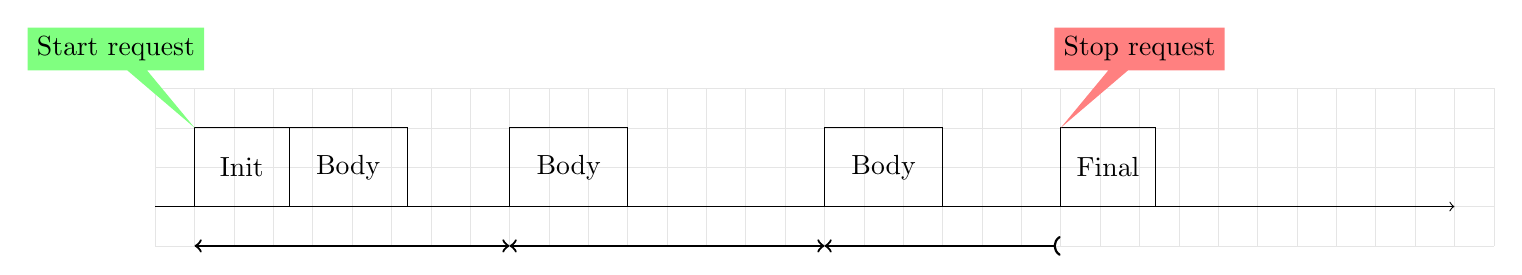
\begin{tikzpicture}
\draw[step=.5cm,gray!20,very thin] (-0.5, -0.5) grid (16.5,1.5);
\draw [->] (-0.5,0) -- (16,0);
\draw (0,0) rectangle (1.2,1);
\node at (0.6,0.5) {Init};
\draw (1.2,0) rectangle (2.7,1);
\node at (1.95,0.5) {Body};
\draw (4,0) rectangle (5.5,1);
\node at (4.75,0.5) {Body};
\draw (8,0) rectangle (9.5,1);
\node at (8.75,0.5) {Body};
\foreach \x in {0, 4}
  \draw [xshift=\x cm,thick,<->] (0,-0.5) -- (4,-0.5); 
\draw [xshift=8 cm,thick,<-(] (0,-0.5) -- (3,-0.5); 
\draw [xshift=11cm] (0,0) rectangle (1.2,1);
\node [xshift=11cm] at (0.6,0.5) {Final};
\node [rectangle callout, fill=green!50, callout absolute pointer={(0,1)}] at (-1,2) {Start request};
\node [rectangle callout, fill=red!50, callout absolute pointer={(11,1)}] at (12,2) {Stop request};
\end{tikzpicture}
\end{adjustbox}
\end{center}


\begin{ex}
Modify the application to take the new requirements into account. Use 3 basic tasks to implement function F. Init and Final simulates the workload by an empty for looping 100 000 times.
\end{ex}

\begin{ex}
Same question but with only one extended task to implement function F.
\end{ex}

\section{Fourth application}

In this part, you will implement a watchdog. It is a mechanism that allows to stop a processing or the waiting for an event when a deadline occurs.

\begin{ex}
In your application, each time `a' is pressed, `b' must pressed within 2 seconds. In such case, you print the time between the two occurrences. Otherwise, an error message is displayed. To simplify, we suppose 2 `a' may not be got within 3 seconds.
\end{ex}

\begin{ex}
What is happening if the timeout occurs just after `b' has been pressed but before the waiting task got the event ? (draw a Gantt diagram of this scenario) If your application does not handle correctly this scenario, modify it.
\end{ex}
\end{document}  
